\subsection{SGBD Utilizado}

O SGBD utilizado é o Maria DB.

Desenvolvido por :
\begin{itemize}
    \item MariaDB Corporation Ab
    \item MariaDB Foundation
    \item Michael 'Monty' Widenius
\end{itemize}

\subsection{Descrição do Projeto}

\begin{FlushLeft}

    \small{

        O Problema Abordado será a gestão de ordens de manutenção.

        Onde terá um processo de manutenção que permita o fluxo correto de trabalho e realizar a compra de materiais para o conserto das máquinas, garantindo o bom funcionamento delas para o operador.

        O Sistema tem um simples controle de usuários, guardando o nome, chapa, senha e email.

        Cada usuário pode ser um operador ou técnico ou comprador, cada um tendo um código único que representa seu cargo.

        Nesse sistema haverá um processo de manutenção que se baseará em notas de manutenção sobre uma máquina, que indicam algum problema ou alerta, ao qual podem virar ordens de manutenção se for crítico.
        Uma Nota, que contem seu código, descrição e a data de criação e se foi rejeitada e seu criador, pode ser criada por um operador que detectou algo incomum ou ser criada sobre uma preventiva de manutenção.

        Quando a nota se torna em uma ordem de manutenção, é definido um novo código para a ordem como a definição de qual tipo de ordem será efetuada, assim tendo um dia de encerramento quando for executada por um operador.

        E assim quando a ordem de manutenção for executada, haverá um consumo de uma material sobre uma máquina.

        Máquina terá seu código, descrição e se é critica. E Material terá seu código, descrição e classificação.

        Para haver o consumo do material sobre uma ordem de manutenção, primeiro é necessário requisitar sua compra, para a realização da compra é criada um Pedido de Compra ao qual será realizada com um comprador.

        Um Pedido de Compra tem o código da compra, data de criação do pedido, data prevista de entrega pelo fornecedor contratado e a data da entrega.

        Quando um pedido de compra é entregue, é feito um relatório dele contento uma descrição sobre o estado da entrega.

        O fornecedor tem o nome, código e localização. O fornecedor fornece materiais, aonde cada um deles tem um preço específico.

        Por fim, máquinas podem precisar de manutenções periódicas, então é definido preventivas, que tem a datas do mês que deve ser executado, sua periodicidade, qual máquina será feita a preventiva, e quem a criou.

        Uma preventiva só pode ser criada por um técnico.
    }
\end{FlushLeft}

\pagebreak

\subsection{Tabelas Criadas}
\begin{FlushLeft}
    \begin{verbatim}
Usuário(pk chapa, senha, email, nome) 
Técnico(pk id,pk fk chapa)
Comprador(pk id,pk fk chapa)
Operador(pk id,pk fk chapa)
Maquina(pk id, descrição, critico)
Material(pk id, descrição, classe)
Fornecedor(pk id, nome)
Preventiva(pk id, fk id_maquina, fk id_tecnico, periodicidade, meses, descrição)
Nota(pk id,fk operador_criador, fk id_maquina, descrição, rejeitado, data de criação)
Ordem(pk id,fk pk id_nota, tipo de ordem, fk id_tecnico, encerramento)
PlanejamentoPreventiva(pk fk id_preventiva,pk fk id_nota)
Fornece(pk fk id_material, pk fk id_fornecedor, preço)
Consumo(pk fk id_material, pk fk id_ordem, pk fk id_maquina, quantidade)
PedidoCompra(pk id, fk id_fornecedor, 
    fk id_comprador, data criação, data de remessa, data de entrada, frete)
Relatório(fk pk id_pedido, descrição)
Requisito(pk fk id_material, pk fk id_ordem, pk fk id_compra, quantidade)
\end{verbatim}
\end{FlushLeft}

\subsection{Diagrama do Banco de Dados}

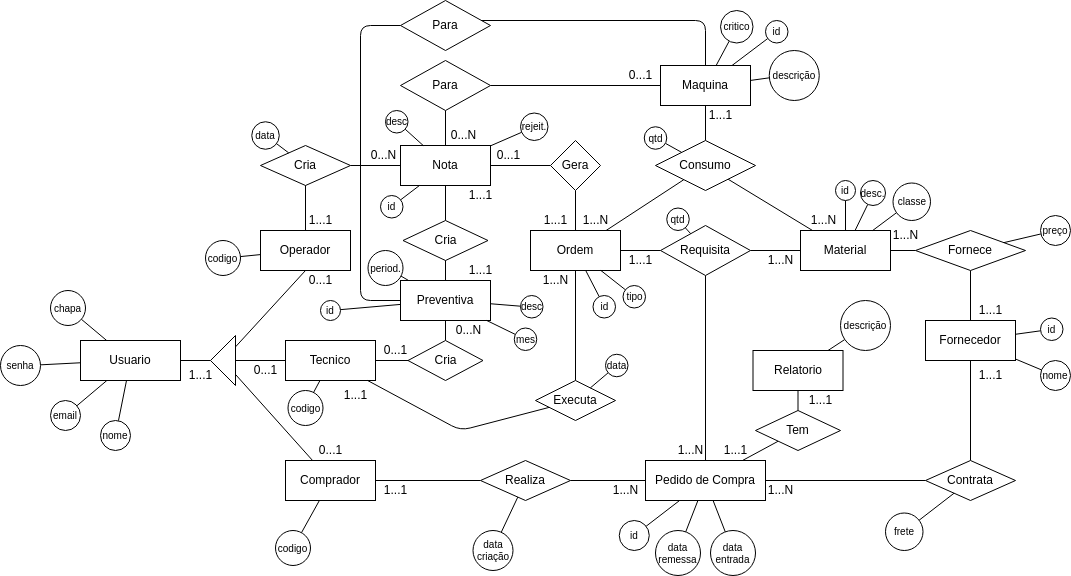
\includegraphics[width=\textwidth]{diagram}


\pagebreak
